\subsection{Punto de equilibrio}

Es necesario calcular el punto de equilibrio ya que permite que la empresa tenga conocimiento de cuantas veces es necesario cubrir los costos fijos de los cuales incurre para sus operaciones. Es importante para determinar en que momento las ventas comenzaran a generar ganancias para la empresa. En la tabla \ref{costosFijosVariables} se proyectan los costos fijos y variables para las ventas del primer año.

\vspace{2mm}
\begin{minipage}{0.9\textwidth}
\centering
\captionof{table}[{Proyección ventas}]{ Proyección ventas. }
\label{costosFijosVariables}
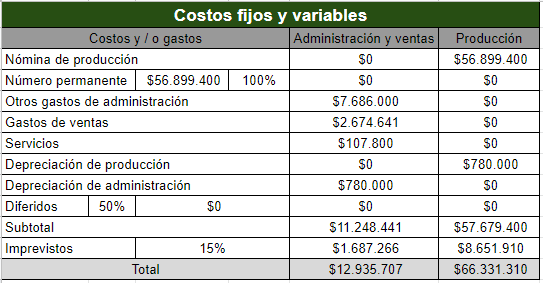
\includegraphics[width=0.9\textwidth]{Images/costosFijosVariables.png}
\fnote{Nota. \textup{Fuente : Autores}}
\end{minipage}

Se calcula el costo fijo de producir cada unidad, agregado el valor de los costos administrativos y ventas se obtiene el valor de costo por unidad. Se proyecta tener un valor agregado del 19\% (\$11.206) de forma que se adquiera el precio de \$70.200, de manera que se deben vender 1122 planes para recuperar la inversión realizada, después de ese tope en adelante sera utilidad.   

\vspace{2mm}
\begin{minipage}{0.9\textwidth}
\centering
\captionof{table}[{Estimaciones punto de equilibrio}]{ Estimaciones punto de equilibrio. }
\label{calculosPuntoEquilirbio}
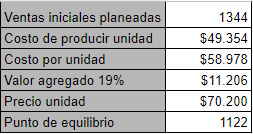
\includegraphics[\textwidth]{Images/estimacion.png}
\fnote{Nota. \textup{Fuente : Autores}}
\end{minipage}

En la gráfica se observa el punto de equilibrio con rectas de costos totales y ventas. En el eje X se encuentran las unidades vendidas y en el eje Y esta la cantidad de dinero, de forma que con 1112 ventas se igualan ambas rectas resultando el punto de equilibrio.

\vspace{2mm}
\begin{minipage}{0.9\textwidth}
\centering
\captionof{figure}[{Gráfica punto de equilibrio. }]{Gráfica punto de equilibrio. }
\label{graficaEquilibrio}
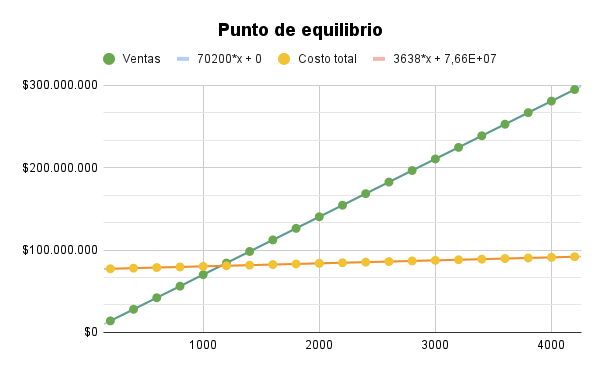
\includegraphics[width=0.9\textwidth]{Images/Punto de equilibrio.png}
\fnote{Nota. \textup{Fuente : Autores}}
\end{minipage}

Teniendo los resultados anteriores en la tabla \ref{puntoEquilibrio} se hace el resumen de la información necesaria para el punto de equilibrio.

\vspace{2mm}
\begin{minipage}{0.9\textwidth}
\centering
\captionof{table}[{Punto de equilibrio}]{ Punto de equilibrio. }
\label{puntoEquilibrio}
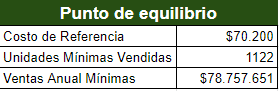
\includegraphics[\textwidth]{Images/tablaPuntoEquilibrio.png}
\fnote{Nota. \textup{Fuente : Autores}}
\end{minipage}